\documentclass[examplethesis.tex]{subfiles}
\begin{document}
\ifxeorlua
\lstdefinestyle{latexExampleForAuthors}{
language=[LaTeX]{TeX},
    breaklines=true,
    postbreak=\mbox{\textcolor{red}{$\hookrightarrow$}\space},
    basicstyle=\small\tt,
    keywordstyle=\color{blue}\sf,
    identifierstyle=\color{magenta},
    commentstyle=\color{cyan},
    backgroundcolor=\color{yellow!15},
    extendedchars=true,
    inputencoding=utf8,
    tabsize=2,
    columns=flexible,
    morekeywords={subtitle, alttitle, altsubtitle, hostcompany, courseCycle,
      courseCode, courseCredits, programcode, degreeName, subjectArea,
      nationalsubjectcategories, todo, ifbiblatex, subsection}
}
\else
\lstdefinestyle{latexExampleForAuthors}{
language=[LaTeX]{TeX},
    breaklines=true,
    postbreak=\mbox{\textcolor{red}{$\hookrightarrow$}\space},
    basicstyle=\small\tt,
    keywordstyle=\color{blue}\sf,
    identifierstyle=\color{magenta},
    commentstyle=\color{cyan},
    backgroundcolor=\color{yellow!15},
    extendedchars=false,
    inputencoding=utf8,
    tabsize=2,
    columns=flexible,
    morekeywords={subtitle, alttitle, altsubtitle, hostcompany, courseCycle,
      courseCode, courseCredits, programcode, degreeName, subjectArea,
      nationalsubjectcategories, todo, ifbiblatex, subsection},
% Support for Swedish, German and Portuguese umlauts
  literate=%
  {Ö}{{\"O}}1
  {Ä}{{\"A}}1
  {Å}{{\AA{}}}1
  {Ü}{{\"U}}1
  {ß}{{\ss}}1
  {ü}{{\"u}}1
  {ö}{{\"o}}1
  {ä}{{\"a}}1
  {å}{{\aa{}}}1
  {á}{{\'a}}1
  {ã}{{\~a}}1
  {é}{{\'e}}1
  {è}{{\`e}}1
  {€}{\euro}1%
  {’}{{\char13}}1
  {-}{{\textendash}}1
  {–}{{\textendash}}1
  {…}{{\ldots}}1,
}
\fi


\chapter{README\_author - the starting place for authors}
\label{ch:READMEauthor}

This document, written by Gerald Q. Maguire Jr, describes the thesis template that I have developed for use at KTH Royal Institute of Technology (KTH). It is important to note that the template is \textbf{not prescriptive}, as not every thesis will have all of the parts that the template shows. However, if there is something that you decide to leave out, you should make a conscious decision to do so and you should consider the impact this may have on your thesis being approved by the examiner.

Fundamental to the design of the template are several key factors:
\begin{itemize}
    \item Helping students be successful in their degree project,
    \item Helping students produce a high-quality thesis, and
    \item Supporting all of the (relevant) phases of the degree project process.
\end{itemize}

\noindent\textbf{This document is a work in progress.}


\section{Advice for Author or Authors}
\label{sec:authors}
One of the hardest problems an author faces is getting started writing, \ie the blank sheet of paper -- empty file barrier. The template provides a \mbox{non-blank} starting point; hence, avoiding the blank paper barrier. Additionally, the template provides some initial structure, basically, an Introduction, Methods, Results, and Discussion (IMRAD) structure, so that there are hints of where to place material. Moreover, there are places (and notes) about material that the student should consider adding; for example, the ``required reflections'' section in the final chapter.

The template (located in the file \texttt{examplethesis.tex}) also provides some examples of commonly occurring types of content, so that one can easily find examples of how to include a figure, table, code listing, \etc. These examples are not meant to be exhaustive and quite often the student will probably need to learn new \LaTeX\  commands in the course of writing their thesis.

As an author, the first step is to configure the \LaTeX\  engine that you will use to process the files - see \Cref{sec:latexEngine}. The second step will be to configure the template - see \Cref{sec:authorConfigs}. The third step will be to make sure that the information about you, your supervisor(s), and the examiner are correct in the file \texttt{custom\_configuration.tex} - this information uses the macros described in \Cref{sec:authorMacros}. Now that you have a lot of the administrative details taken care of it is time to start to write - see \Cref{sec:startingToWrite}.

Note that if you are using Overleaf, it is a good idea to rename the project to a name that includes your name. This will make it easier for your adviser(s) and examiner to find your project in the list of projects they may have in Overleaf.


If you have more detailed questions about the template itself - 
\iflabelexists{ch:READMEnotes}{see \Cref{ch:READMEnotes}.}
{You have to include the \texttt{README\_notes/README\_notes.tex} file when compiling.}

\section{Author configuration of the \LaTeX\  engine}
\label{sec:latexEngine}
The template should work with \textsc{pdfLaTeX}, \XeLaTeX, and \LuaLaTeX.  If you are using Overleaf, I strongly recommend using \XeLaTeX\ ---  as this will get the \texttt{Arial} fonts correct for the KTH cover. If you are running the compiler on your local machine and you use \XeLaTeX\  \textbf{and} you have \texttt{Arial} as a system font, then it will be able to use it. Similarly, for \LuaLaTeX. For \textsc{pdfLaTeX} I have used \textbackslash fontfamily{helvet}, \ie Helvetica, as it is a sans serif font.

One student reported problems with \textsc{fontspec} not loading the fonts properly when running locally with macOS 12.4, TeXLive 2022, LaTeX Workshop on VS Code, and \XeLaTeX\  - the solution is described at \url{https://tug.org/TUGboat/tb39-2/tb122robertson-fontspec.pdf}.

If you are using Overleaf, it is easy to select the compiler (\ie \TeX\ engine) by using the drop-down menu, as shown in \Cref{fig:selectingTeXEngine}.
\begin{figure}[!ht]
  \begin{center}
    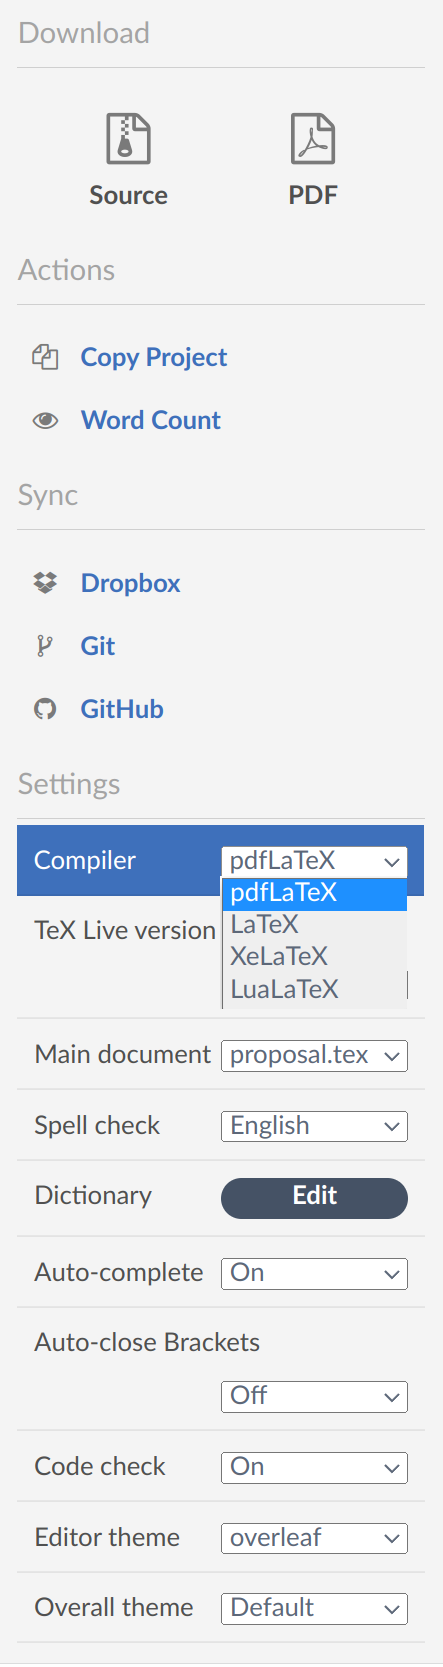
\includegraphics[width=0.40\textwidth]{README_notes/selecting-engine-in-overleaf.png}
  \end{center}
  \caption{Selecting a compiler (\ie TeX engine) in Overleaf}
  \label{fig:selectingTeXEngine}
\end{figure}
\FloatBarrier


\section{Author configuration of the template}
\label{sec:authorConfigs}
The template is designed to handle a thesis written in English or Swedish.
You can set the default language to `english' or `swedish' by passing an option to the documentclass. Note that the language option is written in all lowercase letters; for example, to set the document's language to English:
\begin{lstlisting}[style=latexExampleForAuthors]
\documentclass[english]{kththesis}
\end{lstlisting}

To set the document's language to Swedish (uncomment the following line):
\begin{lstlisting}[style=latexExampleForAuthors]
\documentclass[swedish]{kththesis}
\end{lstlisting}

The language option `swedish' sets the conditional \texttt{\textbackslash ifinswedish} to true.  Among many other things, this conditional is used to configure the KTH cover and the title page to use the chosen language.

The two most common bibliographic engines are supported, \ie BibTeX and BibLaTeX. To set the language to English and use the bibliographic engine to BibTeX you would say:
\begin{lstlisting}[style=latexExampleForAuthors]
\documentclass[english, bibtex]{kththesis}
\end{lstlisting}
To set the language to Swedish and use the bibliographic engine to BibLaTeX you would say:
\begin{lstlisting}[style=latexExampleForAuthors]
\documentclass[swedish, biblatex]{kththesis}
\end{lstlisting}

The above illustrates that you can pass multiple options to the document class separated by commas. Also, note that the options were passed as all lowercase letters.

You can, of course, also modify the formatting of the citations and bibliography. See for example the following code snippet:

\begin{lstlisting}[style=latexExampleForAuthors]
\ifbiblatex
    %\usepackage[language=english,bibstyle=authoryear, citestyle=authoryear, maxbibnames=99]{biblatex}
    %\usepackage[style=numeric,sorting=none,backend=biber]{biblatex}
    \usepackage[bibstyle=authoryear,citestyle=authoryear, maxbibnames=99,language=english]{biblatex}
    % alternatively you might use another style, such as IEEE
    %\usepackage[style=ieee]{biblatex}
    \addbibresource{references.bib}
    %\DeclareLanguageMapping{norsk}{norwegian}
\else
    % The line(s) below are for BibTeX
    \bibliographystyle{bibstyle/myIEEEtran}
    %\bibliographystyle{apalike}
\fi
\end{lstlisting}

To optimize for digital output (this changes the color palette) add the option: \texttt{digitaloutput}. There are also options for A4 or G6 paper: \texttt{a4paper} or \texttt{g5paper} (respectively). The is an option for \texttt{nomenclature}, to produce and refer to equations
\ifnomenclature
as shown in \Cref{ch:NomenclatureExamples}
\fi
.  Finally, there are options for a 1\textsuperscript{st} cycle thesis or 2\textsuperscript{nd} cycle thesis: \texttt{bachelor} and \texttt{master} (respectively); however, these two options are \textbf{not} currently used.

One of the first things that the author(s) will want to do is add the working title and subtitle to the thesis. This is done using the \textbackslash title, \textbackslash subtitle, \textbackslash alttitle, and \textbackslash altsubtitle macros as shown below:
\begin{lstlisting}[style=latexExampleForAuthors]
\title{This is the title in the language of the thesis}
\subtitle{A subtitle in the language of the thesis}

% give the alternative title - i.e., if the thesis is in English,
% then give a Swedish title
\alttitle{Detta är den svenska översättningen av titeln}
\altsubtitle{Detta är den svenska översättningen av undertiteln}
% alternative, if the thesis is in Swedish, then give an English title
%\alttitle{This is the English translation of the title}
%\altsubtitle{This is the English translation of the subtitle}   
\end{lstlisting}

Setting these values once and then using them in many places reduces the work to change them while at the same time ensuring consistency. 

Some additional configuration that the author(s) might do is to set the values of the macros related to the course cycle, course code, date of the thesis, number of credits, degree/exam name, subject area, and if the degree is done external to KTH to set the host information. Consider the snippet below for a student admitted to the ``Bachelor's Programme in Information and Communication Technology (TCOMK)'' program and enrolled in the degree project course ``IA150X Degree Project in Information and Communication Technology, First Cycle 15.0 credits'' and working at a company ``Företaget AB'':
\begin{lstlisting}[style=latexExampleForAuthors]
\hostcompany{Företaget AB} % Remove this line if the project was not done at a host company

\date{\today}

\courseCycle{1}
\courseCode{IA150X}
\courseCredits{15.0}

\programcode{TCOMK}
\degreeName{Bachelors degree}
% Note that the subject area for a Bachelor's thesis (Kandidatexamen)
% should be either Technology or Architecture
% If the thesis is in Swedish, these would be: teknik | arkitektur
% -- Note the use of lower case for the Swedish subject area
\subjectArea{Technology}
\end{lstlisting}

Note that in the above macros you have to give the English or Swedish names in the arguments to \textbackslash degreeName and \textbackslash subjectArea - as shown below:
\begin{lstlisting}[style=latexExampleForAuthors]
\degreeName{Kandidatexamen}
\subjectArea{teknik}
\end{lstlisting}

For a CDATE student enrolled in the course ``DA231X Degree Project in Computer Science and Engineering, Second Cycle 30.0 credits'', the cycle, program, course code, degree, and subject area information would be:
\begin{lstlisting}[style=latexExampleForAuthors]
\programcode{CDATE}
\courseCycle{2}
\courseCode{DA231X}
\courseCredits{30.0}
\degreeName{Degree of Master of Science in Engineering}
\subjectArea{Computer Science and Engineering}
\end{lstlisting}

The set of possible values for the English or Swedish names in the arguments to \textbackslash degreeName are:
\begin{lstlisting}[style=latexExampleForAuthors]
\degreeName{Higher Education Diploma}
\degreeName{Högskoleexamen}

\degreeName{Bachelors degree}
\degreeName{Kandidatexamen}

\degreeName{Master of Architecture}
\degreeName{Arkitektexamen}

\degreeName{Degree of Master of Science in Engineering}
\degreeName{Civilingenjörs}

\degreeName{Magister}
\degreeName{Magisterexamen}

\degreeName{Degree of Master of Science}
\degreeName{Masterexamen}

\degreeName{Master of Science in Engineering and Master of Arts in Education degree}
\degreeName{Civilingenjör och lärare examen}

\degreeName{Degree of Master of Science in Secondary Education}
\degreeName{Ämneslärarexamen}

\degreeName{Both}		# Degree Project in the Field of Technology <teknikområde> and the Main Field of Study <huvudområde>
\degreeName{Same}		# The case when the field of technology <teknikområde> and main field of study <huvudområde> are the same.
\end{lstlisting}

For the last two cases, the code compares the values of subjectArea and secondSubjectArea.

You can find a list of the program codes and school acronyms in the file:\linebreak[4] \texttt{lib/schools\_and\_programs.ins}.

There are a set of rules about what is to be displayed on the KTH cover. These can be found at \url{https://www.kth.se/social/group/sprakkommitten/page/omrade-for-examensarbete/}.

One of the reasons for many of the macros shown above and below is to collect the information that is needed to report the approved thesis in Digitala Vetenskapliga Arkivet (DiVA) and to report the title(s) and grade in \foreignlanguage{swedish}{Lokalt adb–baserat dokumentationssystem (LADOK)}.

National subject categories are a \textbf{required} field in the DiVA record. These categories follow a definition by \foreignlanguage{swedish}{SCB} (nowadays known as \foreignlanguage{swedish}{Statistikmyndigheten} or in English: Statistics Sweden) and HSV (\foreignlanguage{swedish}{Högskoleverket} - nowadays known as  \foreignlanguage{swedish}{Universitetskanslersämbetet (UK-ämbetet)} and \foreignlanguage{swedish}{Universitets- och högskolerådet (UHR)} or in English: Swedish Higher Education Authority and Swedish Council for Higher Education).
While these codes refer to research areas, these codes are also used in KTH to indicate the area of the thesis. The guidance that I received from the Linköping University library was that one should try to use 5-digit codes when possible. Some examples of these codes are shown in Table~\ref{tab:nationalsubject categories}.
\begin{description}[leftmargin=!, labelwidth =\widthof{\texttt{\textbackslash nationalsubjectcategories\{\}}}]
\item [\texttt{\textbackslash nationalsubjectcategories\{\}}] comma separated list of national subject category codes - each a 3 or 5 digit code
\end{description}

\Needspace*{2\baselineskip}
An example for a thesis in Computer Science and Computer Systems:
\begin{lstlisting}[style=latexExampleForAuthors]
\nationalsubjectcategories{10201, 10206}
\end{lstlisting}

You can find the subjects and their codes in:\\ \url{https://www.scb.se/contentassets/3a12f556522d4bdc887c4838a37c7ec7/standard-for-svensk-indelning--av-forskningsamnen-2011-uppdaterad-aug-2016.pdf}\\
and\\
\url{https://www.scb.se/contentassets/10054f2ef27c437884e8cde0d38b9cc4/oversattningsnyckel-forskningsamnen.pdf}

\begin{table}[!ht]
  \begin{center}
    \caption{Examples of some national subject categories and their codes}
    \label{tab:nationalsubject categories}
    \begin{tabular}{p{0.85cm} L{6.2cm} L{6.2cm}} % <-- Alignments: 1st column left, 2nd middle, with vertical lines in between
      \textbf{Code}  & \textbf{Category (in Swedish)} & \textbf{Category (in English)} \\
      \hline
102 & \foreignlanguage{swedish}{Data- och informationsvetenskap (Datateknik)} &   Computer and Information Sciences \\
      \hline
10201 & \foreignlanguage{swedish}{Datavetenskap (datalogi)} & Computer Sciences \\
      \hline
10202 & \foreignlanguage{swedish}{Systemvetenskap, informationssystem och informatik} (\foreignlanguage{swedish}{samhällsvetenskaplig inriktning} under 50804) &
Information Systems (Social aspects to be 50804)\\
      \hline
10203 & \foreignlanguage{swedish}{Bioinformatik (beräkningsbiologi)} (\foreignlanguage{swedish}{tillämpningar} under 10610) & Bioinformatics (Computational Biology) (applications to be 10610) \\
      \hline
10204 & \foreignlanguage{swedish}{Människa-datorinteraktion (interaktionsdesign)} (\foreignlanguage{swedish}{Samhällsvetenskapliga aspekter} under 50803) & Human Computer Interaction (Social aspects to be 50803)\\
      \hline
10205 & \foreignlanguage{swedish}{Programvaruteknik} & Software Engineering \\
      \hline
10206 & \foreignlanguage{swedish}{Datorteknik} & Computer Engineering \\
      \hline
10207 & \foreignlanguage{swedish}{Datorseende och robotik (autonoma system) }& Computer Vision and Robotics (Autonomous Systems) \\
      \hline
10208 & \foreignlanguage{swedish}{Språkteknologi (språkvetenskaplig databehandling)} & Language Technology (Computational Linguistics) \\
      \hline
10209 & \foreignlanguage{swedish}{Medieteknik} & Media and Communication Technology \\
      \hline
10299 & \foreignlanguage{swedish}{Annan data- och informationsvetenskap} & Other Computer and Information Science \\
      \hline
      \hline
202   & \foreignlanguage{swedish}{Elektroteknik och elektronik} & Electrical Engineering, Electronic Engineering, Information Engineering \\
      \hline
20201 & \foreignlanguage{swedish}{Robotteknik och automation} & Robotics \\
      \hline
20202 & \foreignlanguage{swedish}{Reglerteknik} & Control Engineering \\
      \hline
20203 & \foreignlanguage{swedish}{Kommunikationssystem} & Communication Systems \\
      \hline
20204 & \foreignlanguage{swedish}{Telekommunikation} & Telecommunications \\
      \hline
20205 & \foreignlanguage{swedish}{Signalbehandling} & Signal Processing \\
      \hline
20206 & \foreignlanguage{swedish}{Datorsystem} & Computer Systems \\
      \hline
20207 & \foreignlanguage{swedish}{Inbäddad systemteknik} & Embedded Systems \\
      \hline
20299 & \foreignlanguage{swedish}{Annan elektroteknik och elektronik} & Other Electrical Engineering, Electronic Engineering, Information Engineering \\
      \hline
    \end{tabular}
  \end{center}
\end{table}



\FloatBarrier



\section{Author macros}
\label{sec:authorMacros}
It is assumed that there can only be 1 or 2 authors. For many years now 2\textsuperscript{nd} cycle theses are expected to only have one author.

For the author or first author, there are a number of macros defined to store information about the author, so that it can later be used in multiple places -- for example, the KTH cover (produced with \texttt{\textbackslash kthcover)}, the title page (produced with \texttt{\textbackslash titlepage}, the ``For DIVA'' section at the end of the thesis (produced with \linebreak[4]
\texttt{\textbackslash divainfo\{pg:lastPageofPreface\}\{pg:lastPageofMainmatter\}}), and possibly a JavaScript Object Notation (JSON) file named \texttt{fordiva.json} produced as a by product of the \texttt{\textbackslash divainfo}. Note that the actual section name has DiVA set in all caps - which hopefully should not occur in the thesis! If the string DiVA set in all caps, does have to appear, then the section heading should be preceded by four euro signs and followed by four more euro signs (as is done this doucment).

The author-related macros are:
\begin{description}[leftmargin=!, labelwidth =\widthof{\texttt{\textbackslash secondAuthorsFirstname\{\}}}]
\item [\texttt{\textbackslash authorsLastname\{\}}] the last name of the author\footnote{Note that the author's name can include a suffix such as ``, Jr.'' or `` Jr.'', i.e., the suffix can be separated with a comma or not -- as the author prefers to write their name.}

\item [\texttt{\textbackslash authorsFirstname\{\}}] the first name of the author

\item [\texttt{\textbackslash email\{\}}] the KTH e-mail address of the author

\item [\texttt{\textbackslash kthid\{\}}] the author's kthid, this generally starts with the string ·``u1'' and is a unique identifier for every KTH user.

% As per email from KTH Biblioteket on 2021-06-28 students cannot have an OrCiD reported for their degree project
\item [\texttt{\textbackslash authorsSchool\{\}}] the value is generally of the form:\linebreak[4] \texttt{\textbackslash schoolAcronym\{EECS\}}. The currently supported school acronyms are: ABE, CBH, EECS, ITM, and SCI. These are defined in the file\linebreak[4] \texttt{schools\_and\_programs.ins}.
\end{description}

If the first author is not in Stockholm, Sweden when the acknowledgements are written, then add that information via the macros described below.
This information will be used when generating the acknowledgements signature. The acknowledgements signature is the text at the end of the acknowledgements and it gives the place where the author(s) is/are when writing the acknowledgements and also gives the date and name(s).
\begin{description}[leftmargin=!, labelwidth =\widthof{\texttt{\textbackslash secondAuthorsFirstname\{\}}}]
\item [\texttt{\textbackslash authorCity\{A City\}}] specify the city

\item [\texttt{\textbackslash authorCountry\{A Country\}}] specify the country

\item [\texttt{\textbackslash authorCityCountryDate\{\}}] pass into this function the month and year for the acknowledgement. This can be a string such as January 2022 or it can be a \LaTeX\  expression, such as \textbackslash MONTH\textbackslash enspace\textbackslash the\textbackslash year.
\end{description}

If there is a second author and the place, month, and year are \textbf{all} the same, then specify the month and year for only the \textbf{first} author:
\begin{lstlisting}[style=latexExampleForAuthors]
\authorCityCountryDate{\MONTH\enspace\the\year}
\end{lstlisting}

If there is a second author and the place is different, then say:
\begin{lstlisting}[style=latexExampleForAuthors]
\authorCityCountryDate{}
\end{lstlisting}
\clearpage

If there is a second author, the macros are:
\begin{description}[leftmargin=!, labelwidth =\widthof{\texttt{\textbackslash secondAuthorsFirstname\{\}}}]
\item [\texttt{\textbackslash secondAuthorsLastname\{\}}] the last name of the 2\textsuperscript{nd} author
\item [\texttt{\textbackslash secondAuthorsFirstname\{\}}] the first name of the 2\textsuperscript{nd} author
\item [\texttt{\textbackslash secondemail\{\}}] the KTH e-mail address of the 2\textsuperscript{nd} author
\item [\texttt{\textbackslash secondkthid\{\}}] the 2\textsuperscript{nd} author's kthid
% As per email from KTH Biblioteket on 2021-06-28 students cannot have an OrCiD reported for their degree project
\item [\texttt{\textbackslash secondAuthorsSchool\{\}}] the school of the 2\textsuperscript{nd} author
\end{description}

If the second author is not in the same place as the first author, then add the relevant information using the macros below.  This information will be used when generating the acknowledgements signature.
\begin{description}[leftmargin=!, labelwidth =\widthof{\texttt{\textbackslash secondAuthorsFirstname\{\}}}]
\item [\texttt{\textbackslash secondAuthorCity\{A City\}}]  specify the city

\item [\texttt{\textbackslash secondAuthorCountry\{A Country\}}] specify the country

\item [\texttt{\textbackslash secondAuthorCityCountryDate\{\textbackslash MONTH\textbackslash enspace\textbackslash the\textbackslash year\}}]  pass into this function the month and year for the acknowledgement
\end{description}

If the second author is the same place as the first author, then comment out or delete the \textbackslash secondAuthorCityCountryDate\{\} as shown below:
\begin{lstlisting}[style=latexExampleForAuthors]
%\secondAuthorCityCountryDate{}
\end{lstlisting}

\section{Starting to write}
\label{sec:startingToWrite}

As you write you will notice "todo" notes in the template. They follow the following conventions:
\begin{lstlisting}[style=latexExampleForAuthors]
\generalExpl{Comments/directions/... in English}
\sweExpl{Text på svenska}
\engExpl{English descriptions about formatting}
\sweExpl{warnings}
\end{lstlisting}


\subsection{Working abstract}
\label{sec:wrtingFirstAbstract}
I generally recommend that every student start by writing a working abstract, this will help you keep your focus. To find where you can start to enter your abstract look in the \textit{examplethesis.tex} file for the line:
\begin{lstlisting}[style=latexExampleForAuthors]
\generalExpl{Enter your abstract here!}
\end{lstlisting}

There is lots of information already in the template to help you with entering text, equations, \etc in your abstract. \textbf{NB} Abstracts are supposed to stand by themselves, this means no footnotes, no cross-references, no figures, no tables, \etc.

I suggest avoiding the use of the defined acronyms in abstracts \ie spell them out rather than using the glossary commands. This is due to the fact that the \texttt{glossaries} package (that is being used to support acronyms) does not directly provide support for multiple languages and because I do not understand how to programmatically create plurals of acronyms in Swedish or other languages. Even in an English abstract, it is desirable to avoid using the glossary commands - as this makes subsequent processing of the abstracts harder - since one has to make sure that the list of acronyms and their definitions are provided to any program that will process this \LaTeX\  source code. For this reason, later versions of this template include the acronyms.tex file after the metadata for DiVA.

\subsection{Structure of the abstracts and summaries}
The basic \LaTeX\  structure for an abstract or summary is shown below (for the case of an English abstract and a Swedish summary \ie sammanfattning):
\begin{lstlisting}[style=latexExampleForAuthors]
\begin{abstract}
  \markboth{\abstractname}{}
\begin{scontents}[store-env=lang]
eng
\end{scontents}

\begin{scontents}[store-env=abstracts,print-env=true]
here is where you abstract goes.
\end{scontents}

\subsection*{Keywords}
\begin{scontents}[store-env=keywords,print-env=true]
% If you set the EnglishKeywords earlier, you can retrieve them with:
\InsertKeywords{english}
% If you did not set the EnglishKeywords earlier then simply enter the comma separate keywords here:
%such as: Canvas Learning Management System, Docker containers, Performance tuning
\end{scontents}
\end{abstract}

\cleardoublepage
\babelpolyLangStart{swedish}
\begin{abstract}
    \markboth{\abstractname}{}
\begin{scontents}[store-env=lang]
swe
\end{scontents}
\begin{scontents}[store-env=abstracts,print-env=true]
Swedish summary goes here
\end{scontents}
\subsection*{Nyckelord}
\begin{scontents}[store-env=keywords,print-env=true]
% SwedishKeywords were set earlier, hence we can use alternative 2
\InsertKeywords{swedish}
\end{scontents}
\end{abstract}
\babelpolyLangStop{swedish}
\end{lstlisting}

It is important to note that the contents of the \texttt{scontents} environment for the abstracts are stored \textbf{verbatim}, \ie the \LaTeX\  is \textbf{not} executed. The reason for this is to be able to later have a program that can manipulate the source \LaTeX\  to convert it to HTML for use in announcements, calendar events, and for DiVA. This means that if you write the following:
\begin{lstlisting}[style=latexExampleForAuthors]
\begin{scontents}[store-env=abstracts,print-env=true]
\input{abstract.txt}
\end{scontents}
\end{lstlisting}
\noindent what will end up in your abstract in the metadata save for DiVA will simply be: \texttt{''\textbackslash input{abstract.tex}''} -- which means that someone will have to cut and paste your actual abstract to insert it into DiVA.

It is also important to that that the following lines:
\begin{lstlisting}[style=latexExampleForAuthors]
\begin{scontents}[store-env=lang]
eng
\end{scontents}
\end{lstlisting}
\noindent \textbf{must} to be before the \texttt{scontents} environment for the abstracts and keywords -- as these lines indicate what language the subsequent abstract and keywords are in. The three-character code used for the language is the ISO 639-2 Code – specifically the "B" (bibliographic) variant of these codes --- as these codes are used in the DiVA metadata to tag what language is used.

\subsection{Acronyms}
\label{sec:addingAcronyms}
You may want to define an acronym to help you with your writing, as this can both reduce the amount of typing and help your reader by providing consistent use of acronyms. The acronyms' definitions can be found in the file \textit{lib/acronyms.tex}. The file contains some examples. I generally try to sort the lines to help find which acronyms I already have defined and keep track of the new one(s) I want to add.

\subsection{Some predefined macros to help when writing}
\label{sec:predefine}

The file \textit{lib/defines.tex} includes some macros that will help you when writing. This includes \textbackslash etc, to give you ``\etc'', \textbackslash eg, \textbackslash ie, and \textbackslash etal.
The file also defines \textbackslash first, \textbackslash Second, ... \textbackslash eighth to give you \first, \Second, \third, ... \eighth. Note that `Second' is written with an initial capital letter to avoid conflict with the unit `second' in the \texttt{siunitx} package.

\subsection{Additional abstract(s)}
\label{sec:additionalAbstracts}

All theses at KTH are \textbf{required} to have an abstract in both \textit{English} and \textit{Swedish}. However, in addition to this, many students want to add abstracts in additional languages. The template comes pre-configured with places for abstracts in several other languages. If there is a language that you want to use that is not already supported, there are directions for how to add an additional language. If there are abstracts in languages that you do not want, please delete them or comment them out (see \Cref{sec:hideComment}).

\subsection{Removing and hiding parts that you do not want}
\label{sec:hideComment}

It is quite likely that you will find parts of the template that you do not want/need. One way of dealing with this is to delete them, and another way is to comment them out. Personally, I like to comment things out, in case I actually do want to be able to read it in the \LaTeX\  file or uncomment it later. To comment out a portion of the file, simply use the following environment:

\begin{lstlisting}[style=latexExampleForAuthors]
\begin{comment}
    **** what you want to comment out ****
\end{comment}
\end{lstlisting}

For example, if you are not interested in the Swedish language \texttt{todo} notes, you can look for lines with ``\textbackslash sweExpl'' in them and comment them out (or delete them).

\subsection{Removing the README\_notes}
At some point you will no longer want this README information. You can remove it by removing the line
\textbackslash include\{README\_notes/README\_notes\} -- from the \textit{examplethesis.tex} file. You can then remove the \textbf{README\_notes} directory.

Unless you are an examiner or an administrator you can delete the file: \texttt{README\_notes/README\_examiner\_notes.tex} and delete the include of this file from near the end of the template (\ie \textit{examplethesis.tex}. You can also delete the directory \textbf{README\_notes/README\_examiner-figures}.


\section[Copyright or Creative Commons License]{Copyright or Creative Commons\\ License}
\label{sec:copyrightOrCClicense}
It is possible to have several variants of the bookinfo page\footnote{When printed double sided, the bookinfo page is the back of the title page.}:
\begin{enumerate}[labelwidth =\widthof{\textbf{Creative Commons (CC)}}, leftmargin = !]
    \item[copyright] If you want to have a bookinfo page, include the line saying \textbackslash bookinfopage.
    \item[Creative Commons (CC)] If you want to have a bookinfo page but want to have a Creative Commons license, then include \textbackslash bookinfopage and use and configure the \texttt{doclicense} package as described below.
    \item[none] If you do \textbf{not} want to have a bookinfo page, comment the line saying \textbackslash bookinfopage and add a \textbackslash cleardoublepage.
\end{enumerate}

For background about Creative Commons licenses, see:
\url{https://www.kb.se/samverkan-och-utveckling/oppen-tillgang-och-bibsamkonsortiet/open-access-and-bibsam-consortium/open-access/creative-commons-faq-for-researchers.html} and \url{https://kib.ki.se/en/publish-analyse/publish-your-article-open-access/open-licence-your-publication-cc}.

Note that the lowercase version of the Creative Commons license has to be used in the modifier, \ie one of: by, by-nc, by-nd, by-nc-nd, by-sa, by-nc-sa, or zero. For the list of supported licenses, see the documentation for the \texttt{doclicense} package.

Note that if the \texttt{doclicense} package is used, it automatically redefines \texttt{\textbackslash bookinfopage} to be \texttt{\textbackslash bookinfopageCC}.

\subsection{Example configuration to have a CC BY-NC-ND license}

\begin{lstlisting}[style=latexExampleForAuthors]
\usepackage[
    type={CC},
    modifier={by-nc-nd},
    version={4.0},
    hyphenation={RaggedRight},
]{doclicense}
\end{lstlisting}

Note that the option ``hyphenation={RaggedRight}'' can be used with the configuration of the package to set the license information with a ragged right margin rather that as a filled and justified paragraph.


\subsection{Example configuration to have a CC BY-NC-ND license with a Euro symbol rather than a Dollar sign}

\begin{lstlisting}[style=latexExampleForAuthors]
\usepackage[
    type={CC},
    modifier={by-nc-nd},
    version={4.0},
    imagemodifier={-eu-88x31},  % to get Euro symbol rather than Dollar sign
    hyphenation={RaggedRight},
]{doclicense}
\end{lstlisting}


\subsection{Example configuration to have a CC0 license}

\begin{lstlisting}[style=latexExampleForAuthors]
\usepackage[
    type={CC},
    modifier={zero},
    version={1.0},
]{doclicense}
\end{lstlisting}

\section{Use of fonts within the thesis}
\label{sec:useOfFontsWithinThesis}

The choice of fonts is a very individual matter and may be affected by the kind of content that you are trying to write, the language that you are writing in, and what you want to convey to your reader. However, some points to keep in mind are:
\begin{itemize}
    \item Use fonts with serifs for the body of your thesis, their presence makes it much easier for your reader.

    \item Use sans serif fonts for headings. This helps your reader distinguish them from the body.

    \item Be very careful when using fonts that are not widely available\footnote{For example, even though it is widely used. not everyone has the Arial font.}. Unless you embed the fonts that you have used, your reader may not see what you want them to see. Ideally, you should embed all fonts -- even if you only embed the subset you use.

    \item Although there are fonts that have a huge number of characters in them, they might not have the characters that you need.

    \item There are also fonts that, although they have a vast number of characters in them, do not have the math table that \LaTeX\ needs to be able to set mathematical content\footnote{An example of such a font is Google's Noto font. Even though it includes a vast number of characters, it lacks a math table -- although there is an awareness of this missing feature}.
\end{itemize}

What can you do when the fonts you use are missing characters that you need to use? One solution is to use a font that has the character(s) that you want and then make use of them in the places that you need to.

\warningExpl{The details of working with different fonts and characters is a rather complex area and not for the faint-hearted. However, if you \textbf{really} want to have specific characters, \XeLaTeX\ and \LuaLaTeX\ have the means to help you realize what you want. }


\end{document}
